\documentclass[12pt]{article}

%% preamble: Keep it clean; only include those you need

% if the below packages cannot be installed automatically, you can 
% download the required .sty files from CTAN and place them in the
% same location as the .tex file (or upload to overleaf in same
% location (folder) in overleaf

\usepackage{amsmath}
\usepackage{mathrsfs}
\usepackage{amsfonts}
\usepackage[margin = 1in]{geometry}
\usepackage{graphicx}
\usepackage{booktabs}
\usepackage{natbib}
\usepackage{setspace} % for doublespacing
\doublespacing

% highlighting hyper links
\usepackage[colorlinks=true, citecolor=blue]{hyperref}


%% meta data

\title{Proposal: Research Project on new method of Stochastic Differential Equation Symbolic Regression and Application in Quantitative Finance}
\author{Jiahua Song\\
  Department of Applied Physics and Applied Mathematics\\
  Columbia University
}

\begin{document}
\maketitle

\paragraph{Introduction and Framework}
\section{Jiahua's research work Declaration}
The Stochastic Differential Equation (SDE) can describe a lot of processes in real world. Once we have a random variable involved, we can try to use SDE to describe its movement over time. However, many of obvious random variables can be seen as not optimal or complex in terms of perturbation to the initial condition. In order to make it simple and still accurate, we developed a new method to find the variables of SDE and mathematically prove that the method is numerically convergent. In this paper, we will focus on a new proposed method for finding SDE given a dataset, called Text-Included-Principle-Component Symbolic Regression (TIPC-SR). For the pre-processing work is necessary, I will also participate the data part partially to make sure the work will be consistent to the work for theory which is my original responsibility. 

\section{Data Part Research Work}
\label{data}
The research project has been separated into three parts. The first part is data part. In the data part, we focus on finding the relevant data in financial market. Specifically, we determine to choose stocks of technology section in the United States of America. Before the technique part, researchers need to use stock selection method to get the stock we need to use, and do the traditional analysis like price $P$ is determined by the traditional variables like Fed rate etc. Then, the researchers need to determine the texts that related to the selected companies in the portfolio, where the portfolio is determined by the stock selection method by my colleagues. Then, The texts has mainly two types, homogeneous and non-homogeneous, which means the different aspects of influence. For example, praising a company in rhetoric words is different from stating the new advances which may help most people more efficiently. After the text task, the news selection for the different texts can cover different groups of people. The coverage is also a study we need to research on. I would suggest a naive idea to use variants or adaptive Bayesian Classifier (BC) to deal with text task, because BC is a generative method which give a probability distribution to forecast the probability of events occurrence. The procedure of task is to use BC to determine the boundary and to classify the text based on homogeneity. After the classification, I would suggest to use the Larry Page's Pagerank method to determine the importance of each news or media among the public. \citet{Page1999ThePC} has a comprehensive demonstration of Pagerank algorithm. There are also some online sources for Pagerank. I find the summary of \citet{Austin_2006} is very concise and applicable. The criterion of homogeneity is also used in Pagerank so that we know one news cites others since they are homogeneous text regardless of origin. The Figure \ref{fig:BC1} is the framework. 
\begin{figure}
    \centering
    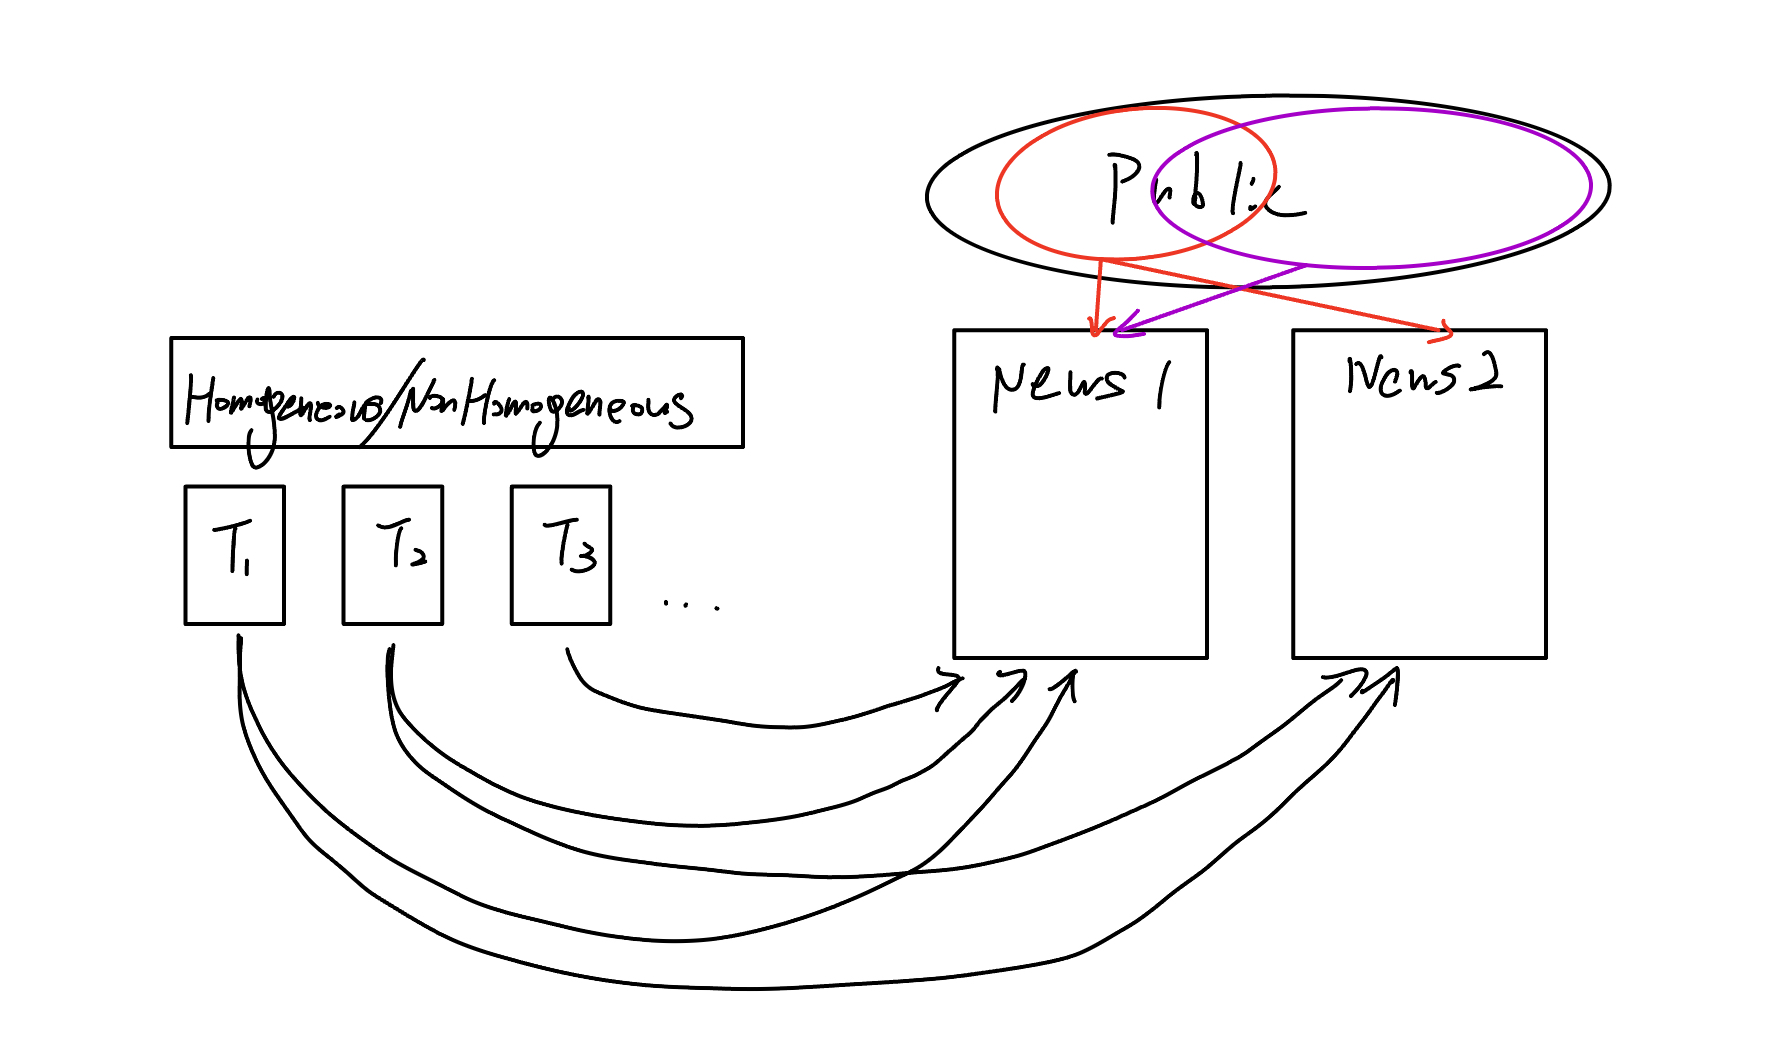
\includegraphics[width=90mm]{Proposal_ Interesting Title/BC1.jpeg}
    \caption{Bayesian Classifier and Pagerank selection for Pre-processing}
    \label{fig:BC1}
\end{figure}

For more details, the research work is open to the researchers in the group. My idea is that we can analyze how the text influences the stock price in each news and analyze all the influential news. The text makes people to make their own decision. Some will buy more at high, low, hold, or sell. The actions will lead stock price to rise and drop by the nature of trading. However, the example is deterministic. The real application should be random, which means the text information will lead a great amount of people to but at high but the number of people is characterized as a random variable or as stochastic process. 

A simple example is that the news can be good or bad for a company. Good has three key types classified by three different homogeneity. We call them 
\[GT1, GT2, GT3,\] 
Same as bad news, we have 
\[
BT1,BT2,BT3,
\]
The price may be affected by these three new variables. 
\[
P(t,GT1, GT2, GT3,BT1,BT2,BT3),
\]where $P$ is price, $t$ is time. Researchers can refine this idea or propose their own idea. The main task of this part is to research on how to use PCA or some other method (like Transformer Architecture) to quantify the text information based on homogeneity. If one determine the method, he needs to immediately discuss with the group of theory part, because the architecture you use may affect the numerical algorithm later discussed in theory part. 

\section{Theory Part Research Work} 
The research topic of my part is on finding optimal SDE fitting the data in financial market. The fundamental principle of optimizing the portfolio is select a set of stocks buy at low price and sell at high price. The difference of price will be the profit range. What we need to do is to maximize the range so that the profit is maximized. 

The range of the stock can be described as one path realization of stochastic process. However, there are thousands of stochastic processes can describe this path. The occurrence of path selected happens to be measure zero in most of cases since the uncountable path can be realized. This is a reason I do not try to find the historical pattern in stock market and try to use and estimation using SDE to predict the stock. Instead of using the numerical information and probability knowledge in this way, I choose to find the {\bf{hidden components}} in the stock market to describe the optimal SDE for fitting. 

\subsection{SDEs}
First of all, the SDE can be apparently described using the obvious components. For example, Geometric Brownian Motion (GBM)
\[
dS_t = \mu S_t \, dt + \sigma S_t \, dW_t
\]
where:
- \(S_t\) is the stock price at time \(t\),\\
- \(\mu\) is the drift coefficient (expected return),\\
- \(\sigma\) is the volatility coefficient (standard deviation of returns),\\
- \(W_t\) is a standard Brownian motion.

\\
Another famous example is the Black-Scholes model. The Black-Scholes model is built upon the GBM and is used for option pricing. The SDE for the underlying stock price in the Black-Scholes model is:
\[
dS_t = \mu S_t \, dt + \sigma S_t \, dW_t
\]
The solution to this SDE is used in the Black-Scholes formula for pricing European call and put options.

\\
Under Ornstein-Uhlenbeck process, we also have Mean-Reverting Models. These models are used for assets that tend to revert to a long-term mean, such as interest rates or commodity prices. For example, 
\[
dX_t = \theta (\mu - X_t) \, dt + \sigma \, dW_t
\]
where:
- \(X_t\) is the process value at time \(t\),\\
- \(\theta\) is the speed of reversion,\\
- \(\mu\) is the long-term mean,\\
- \(\sigma\) is the volatility.

\\
And some others:
Heston Model:
\[
dS_t = \mu S_t \, dt + \sqrt{V_t} S_t \, dW_t^S
\]
\[
dV_t = \kappa (\theta - V_t) \, dt + \xi \sqrt{V_t} \, dW_t^V
\]
where:
- \(S_t\) is the stock price,\\
- \(V_t\) is the variance of the stock price,\\
- \(\kappa\) is the rate of mean reversion of the variance,\\
- \(\theta\) is the long-term mean of the variance,\\
- \(\xi\) is the volatility of the variance,\\
- \(W_t^S\) and \(W_t^V\) are correlated Brownian motions with correlation \(\rho\).
\\
Jump Diffusion Models
\[
dS_t = \mu S_t \, dt + \sigma S_t \, dW_t + S_t \, dJ_t
\]
where \(J_t\) represents the jump process, often modeled as a Poisson process.

\\
Cox-Ingersoll-Ross (CIR) Model
\[
dX_t = \theta (\mu - X_t) \, dt + \sigma \sqrt{X_t} \, dW_t
\]

\subsection{PINN}
\label{pinn}
Physics-informed neural network (PINN) or Physics-informed deep learning is a new topic in machine learning. The fundamentals of PINN originated from the work of Marziar Raissi of Prof. George Karniadarkis' group in 2017 titled: Physics Informed Deep Learning:Data-driven Solutions of Nonlinear Partial Differential Equations \citep{RAISSI2019686}. It was later accepted by the Journal of Computational Physics. The complete work is separated into two main parts. One is an inverse problem; one is a forward problem.

The task of the PINN in solving the inverse problem is to invert the hyperparameters (coefficients) of the terms in the PDE. The setting of this problem means that we do not have real and reliable PDE equations to make a judgment . Therefore, actual observations (values of the field) are needed to provide the loss function. In short, we are picking the best of a family of PDEs to fit the actual system (based on the laws reflected in the actual observations). In order to do this, we need to add these coefficients to the learnable parameters as well so that PINN acts as a player (fitting the PDE system properties) and a referee (finding the best-fitting PDE coefficients to fit).

From a certain point of view, the PINN solving the inverse problem in the original article is not actually a complete solution of the inverse problem because the forward problem is to learn the whole solver, so the corresponding inverse problem should be to learn the whole PDE, not just to compute the coefficients. This is actually a historical limitation because if we want to learn the whole PDE, the operation operators such as addition, subtraction, multiplication, division, and higher-order differentials are not differentiable and cannot be embedded into neural networks. The authors realized at the time that they could not embed these things in a neural network framework. Based on the author's realization of this, his approach takes a back seat. To learn these things, we need to introduce another thing called symbolic learning. Over the years, there have been some interesting things that have broken the previous search explosion logjam, and some interesting things have been done by Dr. Miles Cranmer of Princeton and the previous alphatensor of DeepMind. 

Recently, we found some new methods to combine deep learning with symbolic regression, enabling the possible ways to discover the parametric PDEs from data \citep{Zhang2022DeepLA}. \citet{Zhang2022DeepLA} proposed a method called Parametric Equation Learner (PEQL) to perform neural network-based symbolic regression to parametric equations. The PEQL method is proven to be useful in analyzing systems that we know are partially governed by an analytic equation and partially governed by some other mechanism that may be complex. \citet{PhysRevResearch.4.023174} proposed a Symbolic genetic algorithm (SGA-PDE) method to discover the open-form PDEs directly from data. The framework is that given data and candidates of PDE symbols, we can do a genetic algorithm for binary trees. After crossover, mutation, and replacement, we can get the optimal (measured by the sparse regression) PDE expression governing the given data. The method is successfully tested by finding nonlinear Burger's equation, Korteweg–de Vries equation, and the Chafee-Infante equation \citep{PhysRevResearch.4.023174}. \citet{richterpowell2022neural} proposed a new model called Neural Conservation Laws (NCL) that integrate divergence-free conditions in the neural architecture, ensuring that the continuity equation is always satisfied, thus enabling precise simulation and analysis of fluid dynamics and other related fields. In the industry, the method beats the CFD in the computational sense by avoiding penalty terms. It also enhances the accuracy and reliability of the model in scientific simulations \citep{richterpowell2022neural}.

All of the idea above do not talk about the potential to create the feature space of SDEs. Also, they some of them are limited to the law in previous like NCL. Our work in this part is to design a new PINN method, TIPC-SR, by sound logic and use it in our financial data. The detail of the work includes {\bf{1. create space}}, {\bf{2. design algorithm, numerical analysis on the algorithm for consistency, stability, and convergence (This need to use numerical analysis in math to prove)}}, Itô/Stochastic Calculus to verify the analysis process above is correct as the Itô Calculus analysis is different from the numerical PDE analysis. Researchers can refer to content in \citet{e2019applied}. {\bf{3. Code experiment for simple cases generating SDE.}} The content needs to upload to GitHub. Overall, the TIPC-SR architecture is a sketch for researcher to complete and overcome the difficulties. Here I show a simple framework and example:\\

1. Model Problem: Define the SDE you aim to discover in terms of its components (drift $dt$ and diffusion $dW_t$ terms).\\
2. Neural Network Setup: Construct a neural network where the input is the state and time, and the output optimize the SDE expression.\\
3. Loss Function: Formulate a loss function that includes:\\
   - A data loss term that ensures the neural network output fits the observed data.\\
   - A physics-informed term that ensures the neural network respects the underlying SDE, often incorporating the residuals of the SDE.\\
   - Some other factors that may be applied in Loss function.\\
4. Training: Train the neural network using the combined loss function. The network learns to balance fitting the data and satisfying the differential equation constraints.\\

Example Process:
1. Define the SDE: \[dX_t = b(X_t, t) \, dt + \sigma(X_t, t) \, dW_t\].
2. Construct a neural network with inputs \[(X_t, t)\] and outputs approximating \[b(X_t, t)\] and \[\sigma(X_t, t)\].
3. Define the loss function:
   \[
   \mathcal{L} = \mathcal{L}_{\text{data}} +  \mathcal{L}_{\text{physics}}
   \]
   where \(\mathcal{L}_{\text{data}}\) is the data fitting term and \(\mathcal{L}_{\text{physics}}\) ensures the network satisfies the SDE.

The process of symbolic regression (SR) is similar to PINN framework. SR uses genetic programming as core algorithm to generate SDE. The Figure \ref{fig:PSR} shows the principle of two. However, the interoperability should be argued since intuitively it follows from design but we need to read some papers on this as well. 

\begin{figure}
    \centering
    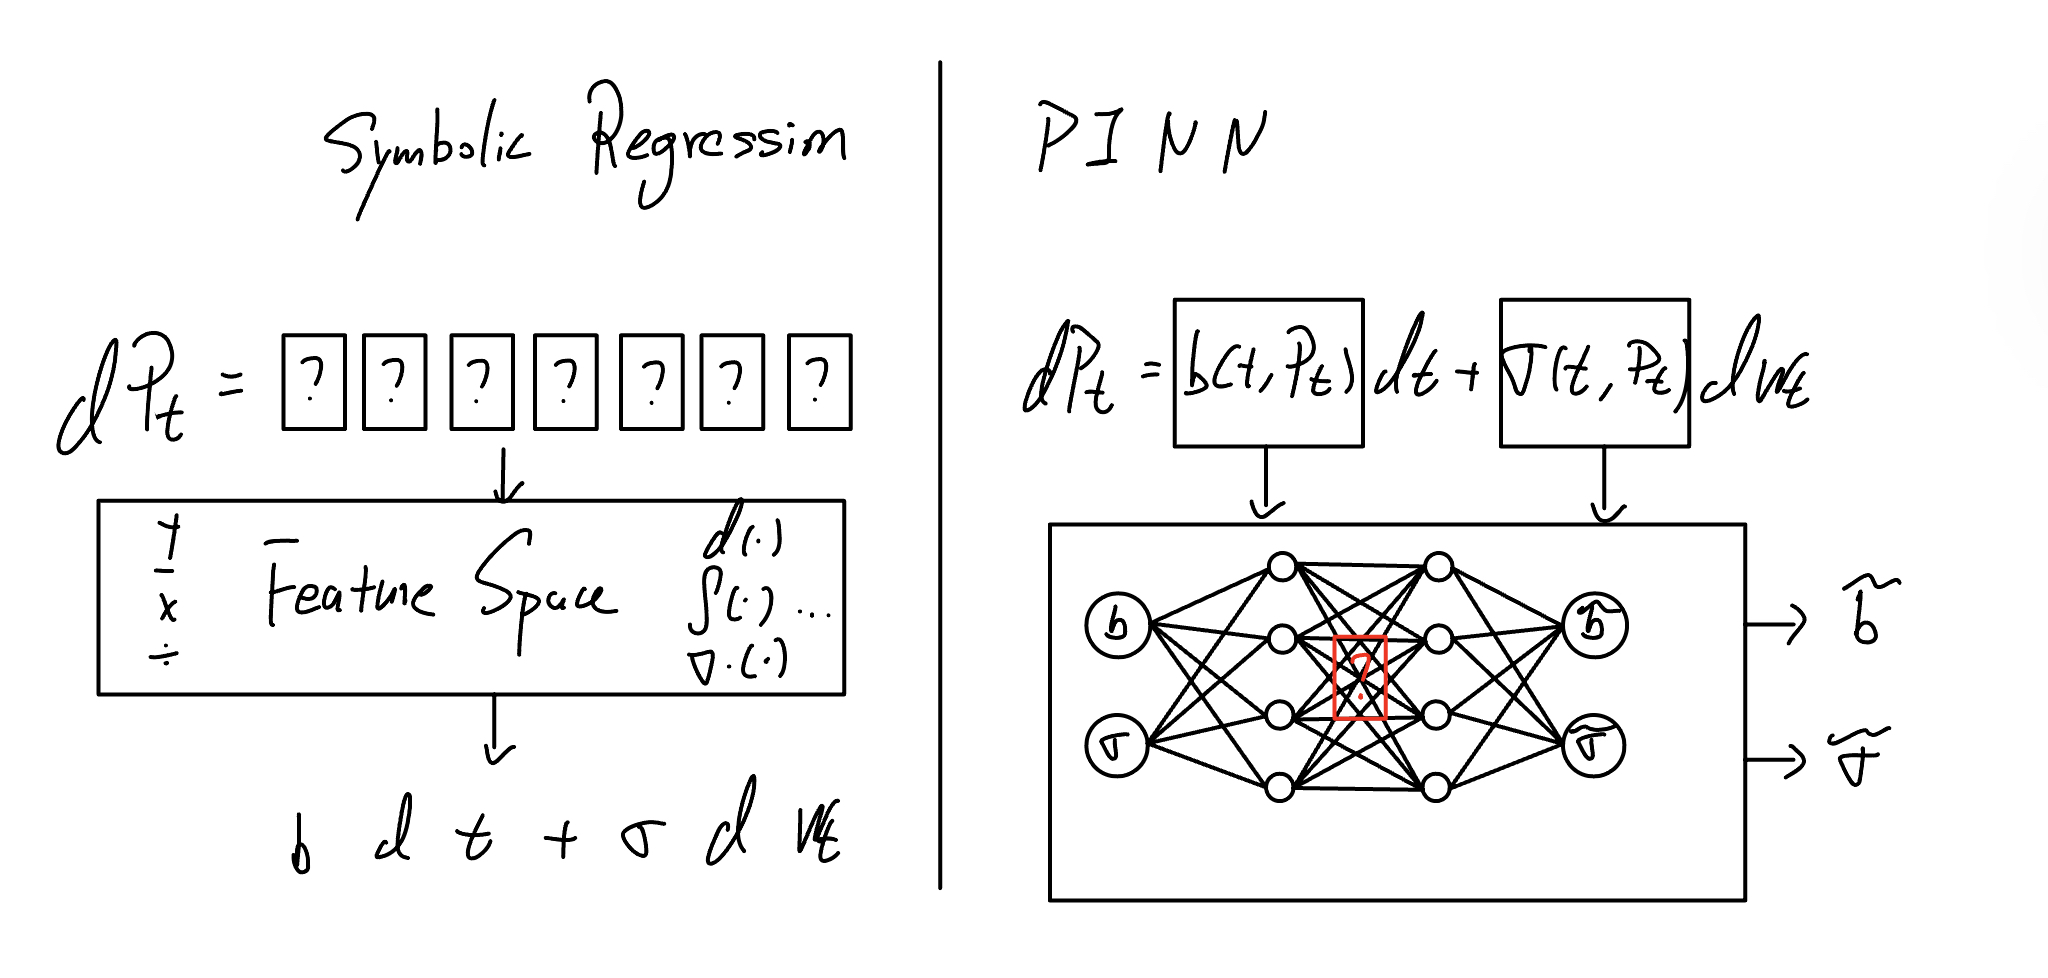
\includegraphics[width=\textwidth]{Proposal_ Interesting Title/PSR.jpeg}
    \caption{PINN and SR}
    \label{fig:PSR}
\end{figure}

After the designing, we do SDE numerical analysis for implementation on computer is guaranteed. We need to build whole architecture of numerical method. It starts from a random initialization set of SDE from feature space. Then, we use the metric we defined in loss function to measure the fitness of each SDE. We order the SDEs and select several (need to argue why this amount) best SDEs in terms of fitness. We do mutation and crossover and pass to the next generation for iteration. We repeat the whole process until the metric gives desirable outcome which is the adjacent solutions are close enough. In principle, if the numerical method is consistent, the solutions can be arbitrarily close. I give a simple example:
Initializing $\{\phi_i\}$, where $\phi_i$ is SDE expressions
\[
\phi_1 \to \phi_2 \to \cdots \to \phi_n
\]
We have the metric from loss function $||\cdot||$ for measurement. Sometimes, SDE involves probability distribution, so wasserstein metric might be used to describe the distance between $\phi_{n-1}$ and $\phi_n$. That is, 
\[
W_p(\psi_{n-1},\psi_{n})=\inf_{\gamma \sim \Gamma(\psi_{n-1},\psi_n)}(\mathbf{E}_{(x,y)\sim \gamma} d(x,y)^p)^{\frac{1}{p}}
\]
where $\psi_i$ is distribution of $\phi_i$. \\
Then, the consistence can be studied. If \[
||\phi_{n}-\phi_{n-1}||\leq \epsilon
\]
where $\epsilon$ is pre-defined, we finished our task. In order to make sure the process and SDEs make sense, stochastic calculus knowledge is needed. Figure \ref{fig:art} shows the whole process. 

\begin{figure}
    \centering
    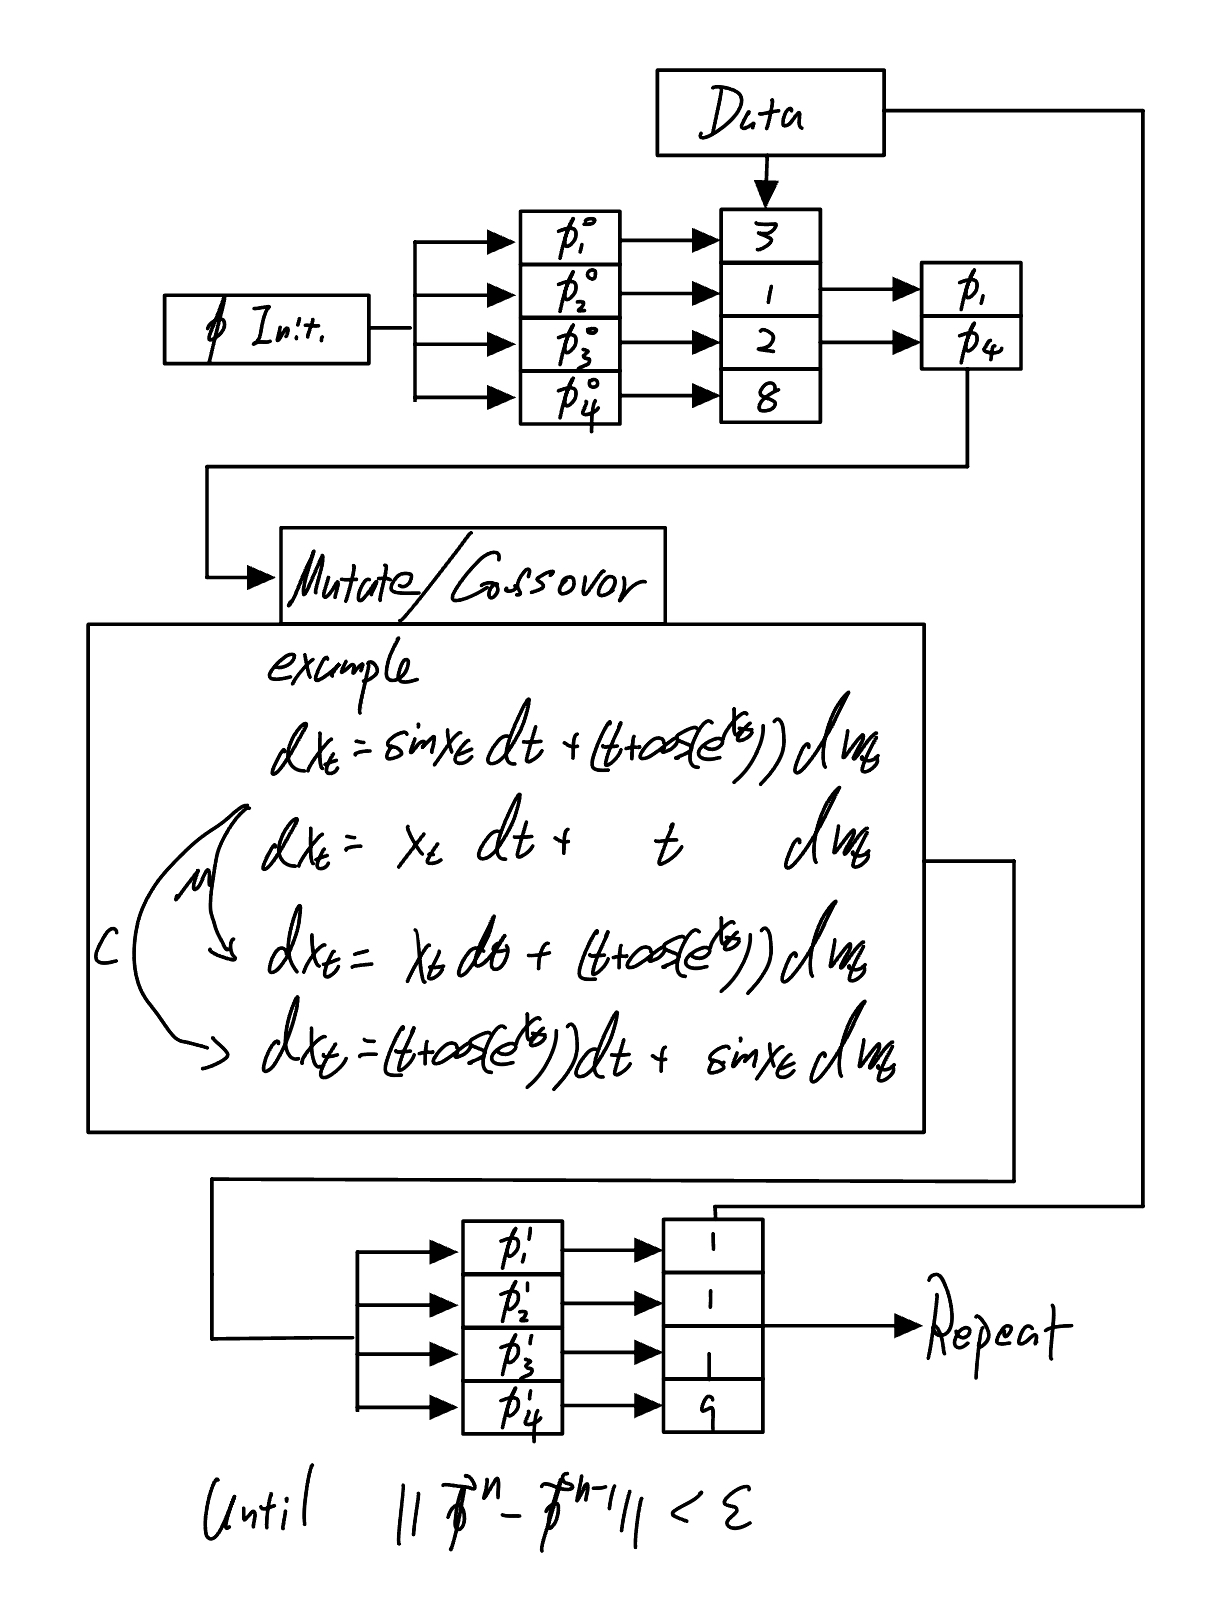
\includegraphics[width=\textwidth]{Proposal_ Interesting Title/art.jpeg}
    \caption{Architecture.}
    \label{fig:art}
\end{figure}

Stability analysis I think is the most intricate part. Once we build the architecture in detail, we can let the whole process to be a neural operator to be studied in math. The numerical stability is needed because when we have some small perturbation in numerical scheme, we have to make sure the solution will not be out of control. The well-posedness of original SDE is critical which is why stochastic calculus is required. The task of stability analysis is to make sure in each iteration the operator norm defined is bounded or in some case less than $1$. For example, let $\mathscr{N}(\cdot)$ be the whole architecture. In each iteration, 
\[
\phi_{n+1}=\mathscr{N}(\phi_n)
\]
is considered. One way to check the stability in numerical sense is to use linearization technique,
\[
\phi_{n+1}=\mathbb{N}(\phi_n)
\]
And the eigenvalues can be calculated for $\mathbb{N}(\cdot)$. 
\[
\phi_{n+1}=\lambda_k(\phi_n)
\]
As $k\to \infty$, $\lambda_k \to \lambda$ which is bounded above by $1$ is desirable to have in this case. However, it sometimes hard to get a bounded operator in this complicated process. Often, the neural operator is weird and unbounded. In this case, I would suggest to use the numerical range method to check the stability. For example, we define
\[
W_H (\mathbb{N})=\{\langle \mathbb{N}x,x\rangle: x\in \mathbb{C}^N, ||x||_H=1\} \text{ on } \ell_{H}^2 (\mathbb{C}^N),
\]
where $H$ is a weight may be identity $I$ or something else for regularization of convergence. As $\mathbb{N} \to \mathscr{N}$, the spectrum (corresponding to the $H=I$) or the numerical range is inside of A-stable region, it will be fine for further explanation of stability. However, if such a condition is not satisfied, we may need to revisit the architecture and think each point in the architecture or use a new stability method to make sure the stability. \\

The whole process of making a consistent and stable method need to be proven by math. The technical detail of math is included in \citet{e2019applied} and some other numerical method textbook. 

\section{Application Part Research Work}
In this part, we proceed in Python or Matlab, and upload into GitHub. The application includes the test mention in \ref{pinn} theory part. We will start from simple experiment. For example, fake and simple space and text to generate SDEs, then make sure it correctly predict the stock price with acceptable error and explanation. Then, we deal with the real data gotten from \ref{data} data part. We need to make sure the SDEs generated can be explained by the whole research reasoning, and the outcome should be useful in real stock market and included in the both research paper and project in GitHub. Researches need to make sure if you have some unsolvable or need time-consuming problem that far exceed or time restriction, they need to move that into discussion and make sure you do not digress from this main topic. 


\bibliography{refs}
\bibliographystyle{asa}

\end{document}